\chapter{Events}
\label{cha:veranstaltungen}

All events mentioned here are also advertised on social media and via posters in the faculty shortly before they actually take place. So check back regularly for detailed information on
Facebook~\link{https://www.facebook.com/iFSR.de/},
Instagram~\link{https://instagram.com/ifsrde},
Twitter~\link{https://twitter.com/ifsr} or on our
website~\link{https://www.ifsr.de}. 
In addition, we also operate a telegram channel~\link{https://t.me/ifsrde}, through which we also keep you up to date.

\minisec{Game nights}

About once a month, the FSR hosts a game night in the APB. It starts at 6:30 pm in the foyer. 
The FSR offers a wide range of games, so that a lot of games are already available. 
If you want to play something that is not there, you can also bring your own games along. Often you can quickly find people to try out a new game.

Every now and then a few people bring their notebooks and throw a small LAN party or bring their game consoles to play together with others via one of the projectors in the seminar rooms.

Nibbles and drinks will be provided, and the \ascii{} is usually open for game nights. 
If the weather cooperates, the student club \emph{Count Down}, is also on site and sells grilled food and alcoholic beverages.

So it's definitely worth stopping by and meeting new people over a mate and a fresh bratwurst or some grilled cheese!



\minisec{Stammtische}

Have you always wanted to get to know your favorite teacher a little more personally? The biannual Stammtisch offers exactly this opportunity. Here you sit down in a relaxed atmosphere with the two participating teachers in a student club and can ask all the questions that have been burning on your tongue for a long time, or perhaps not so long. These are not only technical questions, but also personal ones. The participating teachers are also looking forward to the active participation of the students!

\begin{figure}[b!]
	\centering
  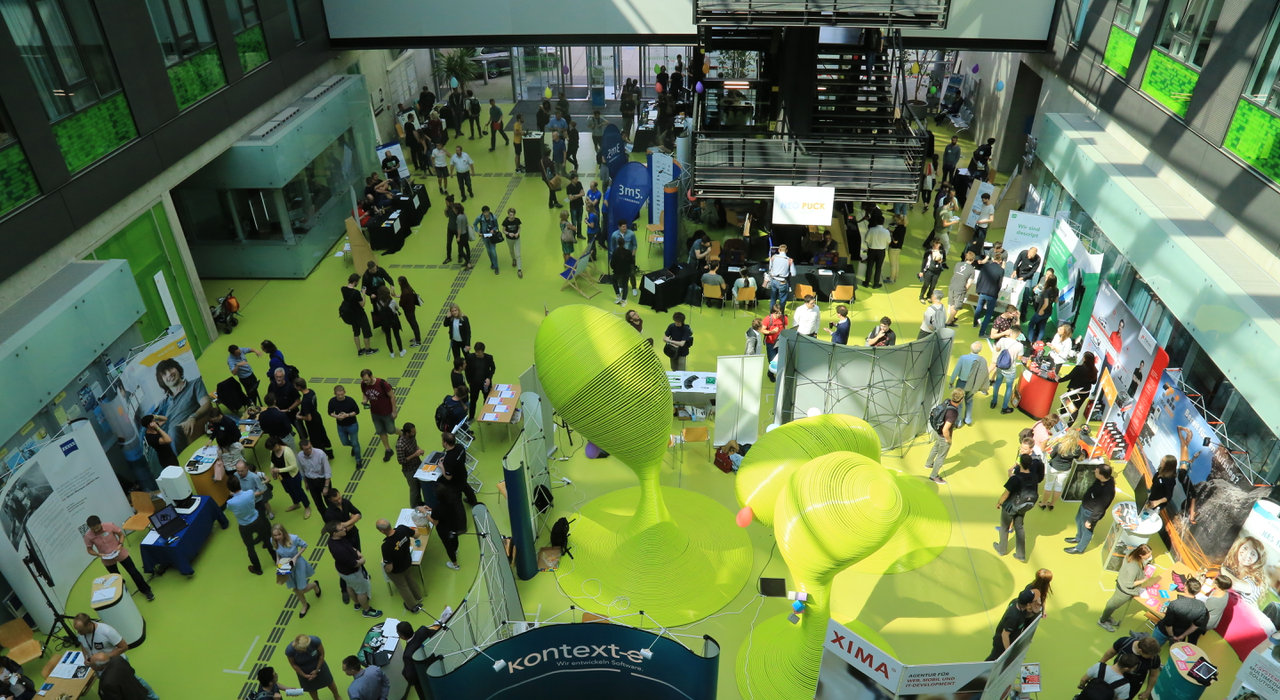
\includegraphics[width=.95\linewidth,keepaspectratio]{img/output.jpg}
  \caption*{\small \centering \textit{OUTPUT\@: Studierende stellen ihre Projekte und Firmen sich selbst vor. -- Foto: Lucas Vogel}}
\end{figure}%

\minisec{Schreibcaf\'e}

You have to write a paper, but you just can't get on with it? 
Help is usually available every Thursday at the \ascii{} Schreibcaf\'e. 
There, writing tutors from the Schreibzentrum will help you with working techniques and feedback to get ahead with your seminar paper or thesis. 
Additionally, there is almost always someone present who can help you with your \LaTeX problems over a cup of coffee.
Due to the current situation regarding Covid-19, the Schreibcaf\'e will not take place weekly and in attendance as usual. 
As soon as this is the case again, you will be informed via our social media and posters in front of the \ascii.
If you need urgent help, you can of course contact the FSR at any time.


\minisec{Dies Academicus}

The Dies Academicus is a lecture-free day where you can get to know other departments and university groups. 
There are workshops, cultural events and much more to get to know the diversity of the campus.

\minisec{Lange Nacht der Wissenschaften}

During the Lange Nacht der Wissenschaften, the university and other research institutions open their doors and prepare an evening program in which they convey what they are working on. Here you can have a look at what is happening in the other areas of the university. Often, the ZIH also offers tours of the thoroughly impressive Rechenzentrum.

\minisec{OUTPUT.DD}

The 
\href{https://output-dd.de}{OUTPUT.DD}
takes place once a year. The stated goal of this event is to present the results of teaching and research to the general public. For this purpose some big companies come to our beautiful faculty and present themselves in the foyer. For you as a student of our faculty this offers \emph{the} chance to familiarize yourself with the companies of the region and to get into conversation with them in an informal setting. This can be a good stepping stone for possible internships or working student jobs. Furthermore, there are often small raffles and contests with prizes for visitors. A visit to OUTPUT is therefore highly recommended. It is worth it!

\minisec{ESE}

The Erstsemestereinführung (ESE) takes place every year at the beginning of October to welcome the new students of our faculty and to introduce them to their studies. 
It is organized by the FSR, which usually starts planning the next ESE shortly after the current one has ended. As you can imagine, this is quite a lot of work, at least if there is no one to help.

This is where you come in. Did you think your ESE was great and want to make sure that all other first-year students have a great ESE as well? Or did you find your ESE absolutely horrible and have a thousand ideas how to make it better? Then get in touch with us at the FSR office and help us with the next iteration of the ESE! We are happy about any help. :)

% \begin{figure}[b!]
%   \centering
%   \includegraphics[width=\linewidth]{img/output_pond}
%   \caption*{\small \centering \textit{Zur OUTPUT wird der Teich zur Lounge -- mit Musik, Freibier und frischem Essen vom Grill. Foto:~Lucas~Vogel}}
% \end{figure}


